 \documentclass[12pt]{article} 
\usepackage[main=portuguese, dutch, english]{babel}
\usepackage[utf8x]{inputenc}
\usepackage{fullpage}
\usepackage{euscript}
\usepackage{amsmath}
\usepackage{amssymb}
\usepackage[amssymb]{SIunits}
\usepackage[pdftex]{graphicx}
\usepackage[colorlinks=true, linkcolor=blue, urlcolor=blue, pdfborder={0 0 0}]{hyperref}
\usepackage{graphics}
\usepackage{subfigure}
\usepackage{float}
\usepackage{caption}
\usepackage{eurosym} 
\usepackage[version=3]{mhchem} 
\usepackage{enumerate}
\usepackage{epsfig}
\usepackage{tikz}
\usepackage{tikzscale}
\usetikzlibrary{babel,arrows,automata}
\usepackage{listings} 
\everymath{\displaystyle} % \frac{}{} tamanho ideal
\usepackage{multirow}
\usepackage{setspace}
\usepackage{indentfirst}
\usepackage{pgfplots}
\usepackage{pdfpages}
\usepackage{comment}
\usepackage[siunitx,american,cuteinductors,smartlabels]{circuitikz}
\usepackage{bodegraph}
\usetikzlibrary{intersections}
\usetikzlibrary{calc}
\usetikzlibrary{positioning}
\usetikzlibrary{arrows}


\usepackage{pdflscape}
\usepackage{fancyhdr} 

\fancypagestyle{mylandscape}{
\fancyhf{} %Clears the header/footer
\fancyfoot{% Footer
\makebox[\textwidth][r]{% Right
  \rlap{\hspace{.75cm}% Push out of margin by \footskip
    \smash{% Remove vertical height
      \raisebox{4.87in}{% Raise vertically
        \rotatebox{90}{\thepage}}}}}}% Rotate counter-clockwise
\renewcommand{\headrulewidth}{0pt}% No header rule
\renewcommand{\footrulewidth}{0pt}% No footer rule
}


 \usepackage[a4paper,left=2cm,right=3cm,top=3cm, bottom = 2cm]{geometry}
%\title{}

\makeatletter
\ctikzset{%
    ly valign/.store in=\ly@valign, ly valign=c,
    ly halign/.store in=\ly@halign, ly halign=l,
}
\ctikzset{ly/.code n args={2}{
  \pgfkeys{/tikz/circuitikz/bipole/label/name=%
        \bgroup
        \setlength{\tabcolsep}{2pt}%
        \def\ly@tabu{\tabular[\ly@valign]}%
        \expandafter\ly@tabu\expandafter{\ly@halign}%
        #1\\ #2%
        \endtabular
        \egroup
    }%
    \ctikzsetvalof{bipole/label/unit}{}
    \ifpgf@circ@siunitx
        \pgf@circ@handleSI{#2}
        \ifpgf@circ@siunitx@res
            \edef\pgf@temp{\pgf@circ@handleSI@val}
            \pgfkeyslet{/tikz/circuitikz/bipole/label/name}{\pgf@temp}
            \edef\pgf@temp{\pgf@circ@handleSI@unit}
            \pgfkeyslet{/tikz/circuitikz/bipole/label/unit}{\pgf@temp}
        \else
        \fi
    \else
    \fi
}}
\ctikzset{ly^/.style args={#1 and #2}{
        ly={#1}{#2},
    \circuitikzbasekey/bipole/label/position=90 }
}
\ctikzset{ly_/.style args={#1 and #2}{
        ly={#1}{#2},
    \circuitikzbasekey/bipole/label/position=-90 }
}

%\let\thetitle\@title
\makeatother


\newcommand{\hoofding}[6]{ 
\begin{flushleft}

\includegraphics[height=3cm]{images/ufrn.png} 
\end{flushleft}
\vspace{-3.3cm} 
\hspace{3cm} 
\parbox{10cm}{#1\\#2\\#3\\#4\\#5\\#6} 
\vspace{-0.6cm}
\hspace{1cm}   

{\parindent=0pt \hrulefill} 
\vspace{0mm}}

\newcommand{\figuur}[2]{\includegraphics[width=#1]{#2}} 
\setlength{\parindent}{25pt}
\setlength{\parskip}{2ex plus 0.5ex minus 0.1ex}


\begin{document}


\hoofding {Universidade Federal do Rio Grande do Norte}{Centro de Tecnologia}{Departamento de Engenharia de Comunicações}{DCO1013 - Comunicações Digitais - 2020.6}{Componentes: Levy Gabriel e Vinicius Malafaya}

\onehalfspacing 

\begin{center}
\large Second laboratory: \textbf{S-parameters and Smith chart}
\end{center}

\setlength{\abovedisplayskip}{-10pt}
\setlength{\belowdisplayskip}{-10pt}

\section{Problem 1}

The objective of this problem is to work with the Smith chart in the ADS. The line characteristic impedance is considered to be $Z_0 = 50 \Omega$

Given $Z = 25 + j30 \Omega$, the normalised impedance is: $\frac{Z}{Z_0} = 0.5 + j0.6$, so the reflection coefficient $\rho_L$ can be found considering the point of intersection between the circle $0.5$ of constant resistance and the circle $0.6$ of constant reactance. So the reflection coefficient a.k.a $S(1,1)$, regarding the S-parameters is: $\rho_L = S(1,1) = -0.149 + j0.46$, according to the figure \ref{p1:smith1} in the marker \textit{rhoL\_1}. 

It is also asked to find the impedance for a $rho_L = 0.5 + j0.1$. Once $\rho_L$ is located according to rectangular coordinates in the complex plane, one way to find the impedance is insert the coordinates $(0.5, 0.1)$ in the complex plane of the Smith chart and observe the normalised impedance obtained, therefore $Z_{\rho_L=0.5 + j0.1} = 2.846 + j0.769$, as seen in the figure \ref{p1:smith1} in the marker \textit{rhoL\_2}.

\begin{figure}[H] 
\centering
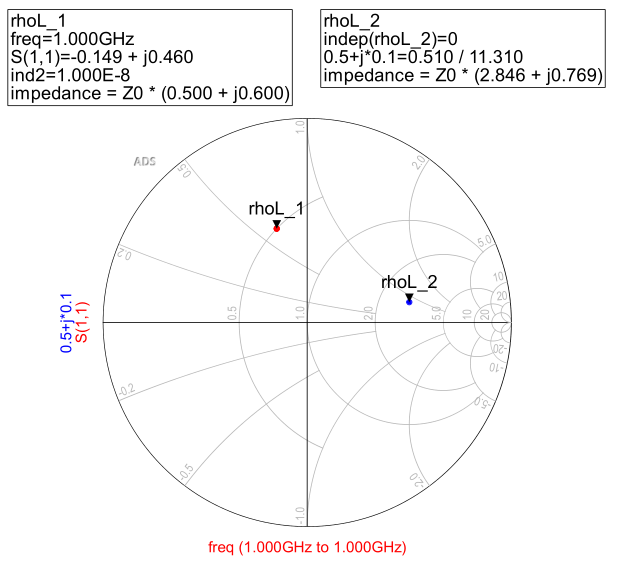
\includegraphics[width=9cm]{images/smith1.PNG}
\caption{Smith chart for the first half of problem 1.}
\label{p1:smith1} 
\end{figure}


The second half of the first problem issues the circuits of the figure \ref{p1:ckts}. In both it is asked to use a frequency of $1 GHz$ and to sweep the values of reactance. 

\begin{figure}[H] 
\centering
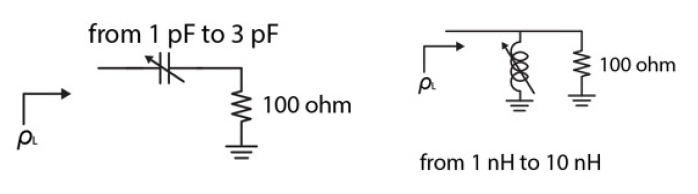
\includegraphics[width=10cm]{images/cktp1.png}
\caption{Circuits for problem 1.}
\label{p1:ckts} 
\end{figure}

The circuit at the left have a capacitor in series with a resistor, when varying the capacitance value, the Smith chart in figure \ref{p1:smith2} (a) will have the reflection coefficients varying in the circle of constant resistance. The figure \ref{p1:smith2} (b) show the same circuit for the admittance chart and it is clearly seen that the circuit behaviour is not easily observed by this kind of chart. 

\begin{figure}[H] 
\centering
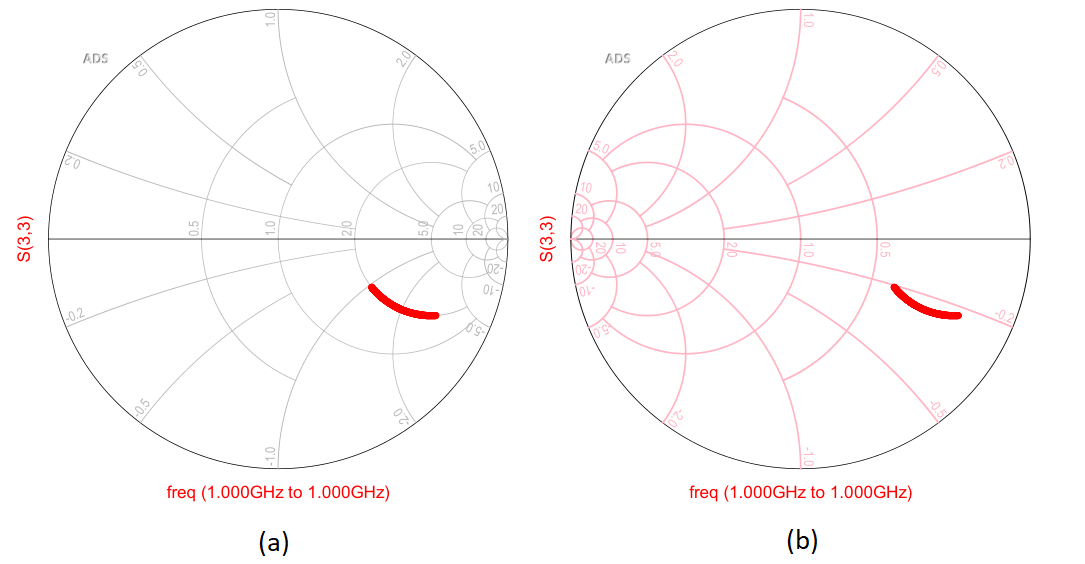
\includegraphics[width=15cm]{images/smith2.png}
\caption{Smith chart for the RC series circuit.}
\label{p1:smith2} 
\end{figure}

On the contrary, the circuit at the right have a inductance in parallel with a resistor and when varying the inductance, a most convenient way to observe the variation of the reflection coefficient is by the admittance chart in the figure \ref{p1:smith3} (a), since the markers walk in the circle of constant conductance.

\begin{figure}[H] 
\centering
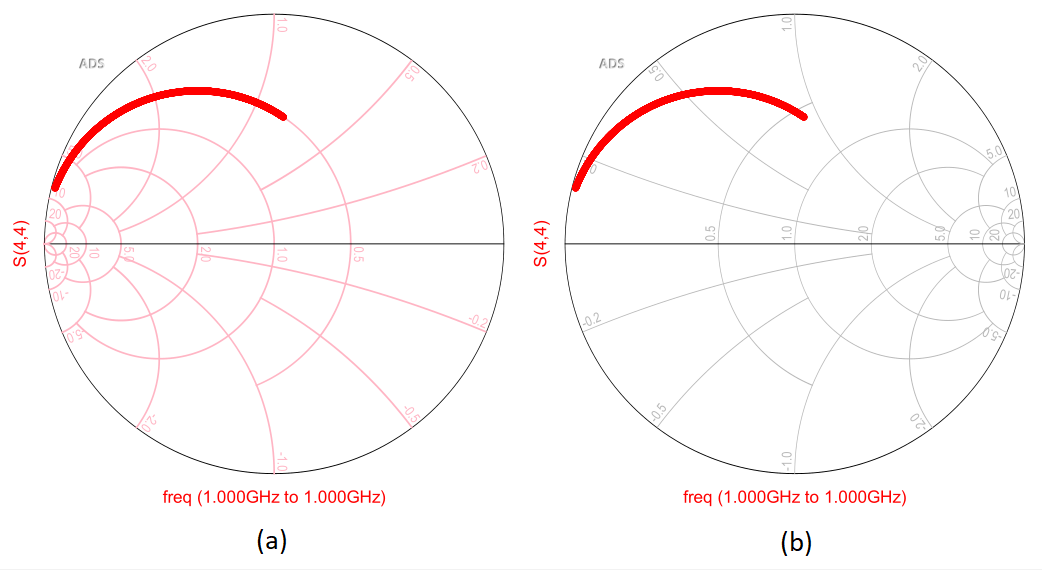
\includegraphics[width=15cm]{images/smith3.png}
\caption{Smith chart for the RL parallel circuit.}
\label{p1:smith3} 
\end{figure}
\section{Problem 2}

This problem address multiples matching networks topologies, still using a L network, but introducing the T network and a multiple sections matching network.

\subsection{Designing the matching network}

The circuit without the matching network is a simple series association of two \texttt{Term}s component representing the source with $R_S = 500 \Omega$ and other representing the load with $Z_L = 50 + j15.9 \Omega$ at $f_o = 1 GHz$.

In a passive component representation, the load impedance can be seen as a series association of a resistance of $R_L = 50 \Omega$ with a inductance of $L_L = X_L/w_o = 2.53 \, nH$. 

Since the input impedance seen from the source must be a higher value than the actual load impedance, the L network in figure \ref{graph:2} will promote a series to parallel impedance transformation in a way that the load impedance seen from the source point-of-view is $R_{in} = R_S$.


\begin{figure}[H]
\centering
\tikz \node [scale=0.8, inner sep=0] {
\begin{tikzpicture} 
    \draw[black, very thick] (-2,3) -- (0,3);
    \draw[black, very thick] (0,3) -- (0,0);
    \draw[black, very thick] (0,0) -- (2,0);
    \node[blue] at (-2.4,3) {$R_{in}$};  
    \node[red] at (2.4,0) {$R_{L}$};  
    \node[black] at (1,1.5) {$1+Q_s^2$};  
    \draw[>=latex, <->] (0.2,0) -- (0.2,3);
    \node[black] at (0,-0.5) {(a)};
\end{tikzpicture}
};
\hspace{1cm}
\tikz \node [scale=0.8, inner sep=0] {
\begin{tikzpicture} [american]
    \draw[>=triangle 90, ->] (-0.5,0) -- (0.5,0);
    \draw[>=triangle 90, ->] (6.5,0) -- (5.5,0);
    \node[black] at (-0.9,0) {$R_{in}$}; 
    \node[black] at (6.9,0) {$R_L$}; 
    \node[black] at (3,-4) {(b)};
    \draw (1,0) to[L, l=$L$, *-*] (5,0)
    (2,0) to[C, l=$C$, *-] (2,-3) node[ground]{}
    ;
\end{tikzpicture}
};

\caption{(a) Desired effect of impedance gain(b) L matching network for a serial to parallel transformation of load impedance. Source: own.}
\label{graph:2} 
\end{figure}

This circuit differs from the previous because it introduces a inductance in the load impedance. But this does not present any problem, since the network of figure \ref{graph:2} introduces a inductor in series with the load and its value can be found disregarding  the load inductance and after concluding the project, the load inductance can be deducted from the network inductance.

As seen in figure \ref{graph:2}(a), the impedance gain must amplify the value of the load impedance such in equation \ref{eq:6}.

\begin{equation} \label{eq:6}
    R_{in} = R_L(1+Q_s^2)
\end{equation}

The quality factor for the series association is \ref{eq:7}:

\begin{equation} \label{eq:7}
    Q_s = \sqrt{\frac{R_in}{R_{L}}-1} = 3
\end{equation}

Since the inductance of the matching network is in a series association with the load, the series quality factor is also found as the relation between the reactance with the resistance, resulting in a expression for the network inductance \ref{eq:8}.

\begin{equation} \label{eq:8}
    Q_s = \frac{L\omega_o}{R_L} \Longrightarrow L = \frac{Q_sR_L}{\omega_o} = 23.87 \, nH
\end{equation}

To calculate the network capacitance we need to transform the parallel L portion in a RLC series association, transforming L in its series equivalent with equation \ref{eq:9}.

\begin{equation} \label{eq:9}
    L_s = \frac{L}{1+Qp^{-2}} = 26.53 \, nH
\end{equation}

The capacitance can be easily found by the resonance frequency expression \ref{eq:10}.

\begin{equation} \label{eq:10}
    \omega_o = \frac{1}{\sqrt{L_sC}} \Longrightarrow C = \frac{1}{L_s \omega^2} = 0.9549 \, pF
\end{equation}

Yet the true value of L was not found, and its results from subtracting the load inductance $L_L = 2.53 \, nH$ from the result in \ref{eq:8}, so we have $L = 21.34 \, nH$.

The figure \ref{fig:smith4} illustrates the smith chart representing a match ($|S_{11}| \approx 0$) and the input impedance corresponding to the new source impedance $Z_{in} \approx 500 \Omega$ at $1 GHz$.

\begin{figure}[H] 
\centering
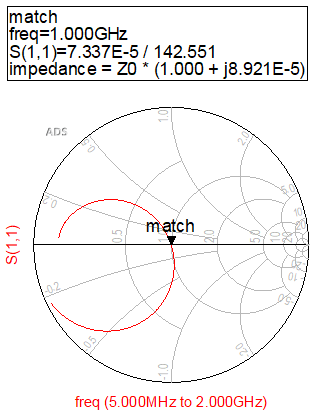
\includegraphics[width=7.5cm]{images/smith4.PNG}
\caption{Circuit $R_S=500 \Omega$ and $R_L=50 \Omega$ with matching network.}
\label{fig:smith4} 
\end{figure}

As a matter of comparison on future topics, we have designed a second L type matching network for a circuit with $R_S=20 \Omega$, $R_L=100 \Omega$ and $f_o = 10 GHz$ using the same methodology as before and same matching network topology (like in figure \ref{graph:1}), with quality factor $Q = 2$, inductance $L = 0.7958 \, nH$ and capacitance $C = 0.3979 \, pF$.

\subsection{Bandwidth comparison of matching network topologies}

This section will compare the previous circuit bandwidth with new impedance matching networks. Aiming an easy design for these additional networks, we will use the ADS impedance match tool \texttt{Impedance Matching}. The additional networks will obey the specifications below:

\begin{itemize}
    \item T-network with intermediate impedance $R_i = 1 k \omega$;
    \item T-network with intermediate impedance $R_i = 5 k \omega$;
    \item Low-Q three sections network;
\end{itemize}

Both the T-networks were designed using two L-network impedance match blocks in a cascade association, carefully choosing the corresponding intermediate impedance of each block to correspond the specification.

It is interesting to see that both intermediate impedances from the T-networks have higher values than input impedance. Also the input impedance is higher than the load impedance. This allow us to analyze that the impedance gain in the L-section close to the load is higher than the other section and the input impedance behaviour is to rise above the desired value and drop to the source impedance. This design pattern can be observed in the figure \ref{graph:3}. For a higher bandwidth the designer would want a minimum rise in the impedance in each section that allow a low-Q.


\begin{figure}[H]
\centering
\tikz \node [scale=0.8, inner sep=0] {
\begin{tikzpicture} 
    \draw[black, very thick] (-2,1) -- (0,1);
    \draw[black, very thick] (0,1) -- (0,3);
    \draw[black, very thick] (0,3) -- (2,3);
    \draw[black, very thick] (2,3) -- (2,-1);
    \draw[black, very thick] (2,-1) -- (4,-1);
    \node[blue] at (-2.4,1) {$R_{in}$};  
    \node[red] at (4.4,-1) {$R_{L}$}; 
    \node[black] at (1,3.4) {$R_{i}$}; 
    \node[black] at (-1.2,2) {$1+Q_2^2$}; 
    \node[black] at (3.2,1) {$1+Q_1^2$}; 
    \draw[>=latex, <->] (-0.2,1) -- (-0.2,3);
    \draw[>=latex, <->] (2.2,-1) -- (2.2,3);
    \node[black] at (0,-1.5) {(a)};
\end{tikzpicture}
};
\hspace{1cm}
\tikz \node [scale=0.8, inner sep=0] {
\begin{tikzpicture} [american]
    \draw[>=triangle 90, ->] (-2.5,0) -- (-1.5,0);
    \draw[>=triangle 90, ->] (6.5,0) -- (5.5,0);
    \draw[] (2,0.3) -- (2,0.8);
    \draw[>=triangle 90, ->] (2,0.3) -- (2.5,0.3);
    \node[black] at (2,1.2) {$R_{i}$}; 
    \node[black] at (-2.9,0) {$R_{in}$}; 
    \node[black] at (6.9,0) {$R_L$}; 
    \node[black] at (2,-4) {(b)};
    \draw (2,0) to[L, l=$L_1$, *-*] (5,0)
    (2,0) to[C, l=$C$, *-] (2,-3) node[ground]{}
    (-1,0) to[L, l=$L_2$, *-*] (2,0)
    ;
\end{tikzpicture}
};

\caption{(a) Desired effect of impedance gain(b) T matching network for a serial to parallel transformation of load impedance. Source: own.}
\label{graph:3} 
\end{figure}

The low-Q three sections network is more complex since it has two intermediate impedance and these have to be found to minimize the steps in the input impedance in each given L-network, therefore ensuring the low-Q characteristic. Once we are using the ADS tool for impedance matching, there is only the need to find the set of intermediate impedance. 

The overall low-Q three sections network is as seen in figure \ref{graph:4}. 


\begin{figure}[H]
\centering
\tikz \node [scale=0.7, inner sep=0] {
\begin{tikzpicture} 
    \draw[black, very thick] (-2,3) -- (-1,3);
    \draw[black, very thick] (-1,3) -- (-1,2);
    \draw[black, very thick] (-1,2) -- (0,2);
    \draw[black, very thick] (0,2) -- (0,1);
    \draw[black, very thick] (0,1) -- (1,1);
    \draw[black, very thick] (1,1) -- (1,0);
    \draw[black, very thick] (1,0) -- (2,0);

    \node[blue] at (-1.5,3.4) {$R_{in}$};  
    \node[red] at (1.5,0.4) {$R_{L}$}; 
    
    \node[black] at (-0.5,2.4) {$R_{i1}$};
    \node[black] at (0.5,1.4) {$R_{i2}$};
    
    \node[black] at (2.7,2.5) {$1+Q_3^2$}; 
    \node[black] at (2.7,1.5) {$1+Q_2^2$};
    \node[black] at (2.7,0.5) {$1+Q_1^2$};
    
    \draw[>=latex, <->] (2,3) -- (2,2);
    \draw[>=latex, <->] (2,2) -- (2,1);
    \draw[>=latex, <->] (2,1) -- (2,0);
    \node[black] at (0,-0.5) {(a)};
\end{tikzpicture}
};
\hspace{1cm}
\tikz \node [scale=0.7, inner sep=0] {
\begin{tikzpicture} [american]
    \draw[>=triangle 90, ->] (-5.5,0) -- (-4.5,0);
    \draw[>=triangle 90, ->] (6.5,0) -- (5.5,0);
    \draw[] (2,0.3) -- (2,0.8);
    \draw[>=triangle 90, ->] (-1,0.3) -- (-0.5,0.3);
    \draw[] (-1,0.3) -- (-1,0.8);
    \draw[>=triangle 90, ->] (2,0.3) -- (2.5,0.3);
    \node[black] at (2,1.2) {$R_{i1}$}; 
    \node[black] at (-1,1.2) {$R_{i2}$}; 
    \node[black] at (-5.9,0) {$R_{in}$}; 
    \node[black] at (6.9,0) {$R_L$}; 
    \node[black] at (0.5,-4) {(b)};
    \draw (2,0) to[L, l=$L_1$, *-*] (5,0)
    (2,0) to[C, l=$C_1$, *-] (2,-3) node[ground]{}
    (-1,0) to[L, l=$L_2$, *-*] (2,0)
    (-1,0) to[C, l=$C_2$, *-] (-1,-3) node[ground]{}
    (-4,0) to[L, l=$L_3$, *-*] (-1,0)
    (-4,0) to[C, l=$C_3$, *-] (-4,-3) node[ground]{}
    ;
\end{tikzpicture}
};

\caption{(a) Desired effect of impedance gain(b) Low-Q three sections network. Source: own.}
\label{graph:4} 
\end{figure}

The total gain correspond to the relation between input and output impedance:

\begin{equation} \label{lQ:1}
    m_{tot} = \frac{R_{in}}{R_L} = \frac{500}{50} = 10
\end{equation}

Once we are using a three section matching network ($n=3$), the impedance gain in each section will be equal in between them and equal to the cube root of the total gain:

\begin{equation} \label{lQ:2}
    m = m_1 = m_2 = m_3 = \sqrt[n]{m_{tot}} = \sqrt[3]{10} = 2.1544
\end{equation}

So after each step the corresponding intermediate impedance and, therefore the input impedance will be:

\begin{equation} \label{lQ:3}
    \begin{aligned}
        R_{i1} = m R_L = 107.72 \, \Omega \\
        R_{i2} = m R_{i1} = 232.07 \, \Omega \\
        R_{in} = m R_{i2} = 500 \, \Omega 
    \end{aligned}
\end{equation}

The same reasoning can be applied for a matching network of p-th order.

Simulating all four networks together we obtain the graph in the figure \ref{fig:bw3}. The first simulation regarding $S(2,1)$ in a solid red line refers to the first matching network designed in the begin of this problem and it is a L-network. Looking to the two T-networks with different intermediate impedances, one regarding $S(4,3)$ with a dot-dash black line and $R_i = 1 k\Omega$ and the another network regarding $S(6,5)$ with a dashed blue line and $R_i = 5 k\Omega$. We can see that the T-network insert a degree of freedom to manipulate the quality factor (therefore the bandwidth) without changing the impedance gain. This degree of freedom is does not exist in the L-network, so this topology do not allow a change in the bandwidth without changing the impedance gain.

When we rose the intermediate impedance from $1k\Omega$ to $5k\Omega$ in the T-network the bandwidth of the transmission coefficient became narrow, this is because we rose the quality factor turning the matching network more selective to the desired frequency.

\begin{figure}[H] 
\centering
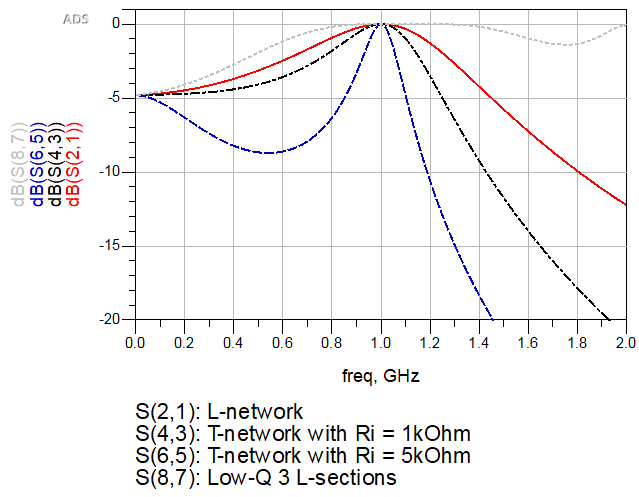
\includegraphics[width=8cm]{images/BW3.PNG}
\caption{Circuit $R_S=500 \Omega$ and $R_L=50 \Omega$ with four different matching networks.}
\label{fig:bw3} 
\end{figure}

In the plot for the low-Q three L-sections network, regarding $S(6,5)$ with dotted cyan line, we can see a different effect from the one obtained before rising the intermediate impedances. In this case the bandwidth rose, since we are ensuring a low-Q.

The effect of a large or narrow bandwidth depends on application specifics and how to achieve this bandwidth is a matter of design to choose the ideal matching network topology to ensure a high quality product and lowest cost.

\section{Problem 3}

This problem takes into account the transmission line in figure \ref{p3:TL}. The circuit illustrates a power amplifier (non-ideal voltage source with impedance $Z_S$) that feeds an antenna (load) with impedance $Z_L = 50 \Omega$ through a transmission line with characteristic impedance $Z_0=50 \Omega$, length $l=21.875 cm$ and relative permittivity of $\epsilon_r=4$ (the relative permeability is considered to be unitary $\mu_r = 1$). Additional information was achieved from measurements with a capacitive probe, they are:


\begin{itemize}
    \item As getting far from the load the voltage drops and reach a minimum at $4.75 mm$ of distance from the antenna;
    \item Beyond this point the voltage rises and reach its maximum at $36 mm$ of distance from the antenna with $\text{VSWR}=3$.
\end{itemize}

\begin{figure}[H] 
\centering
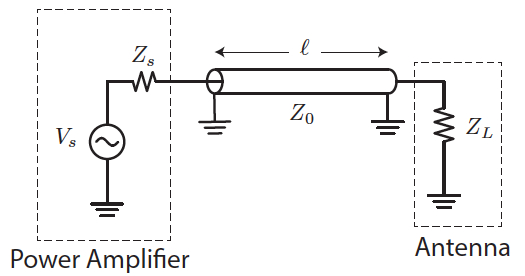
\includegraphics[width=9cm]{images/tl_ckt_p3.png}
\caption{Transmission line for problem 3.}
\label{p3:TL} 
\end{figure}

\subsection{Power amplifier operating frequency}

It known that the distance between the maximum voltage and its minimum is equivalent to a quarter of wavelength, so: $\Delta z = z_{max} - z_{min} = \frac{\lambda}{4} = 31.25mm$ and finally $\lambda = 125mm$. Therefore the operating frequency is given by equation \ref{p3:opfreq}: 

\begin{equation} \label{p3:opfreq}
    f = \frac{v}{\lambda} = \frac{c}{\lambda} \frac{1}{\sqrt{\epsilon_r \mu_r}} = \frac{3 \times 10^8}{125 \times 10^{-3}} \frac{1}{\sqrt{4 \times 1}} = 1.2 GHz
\end{equation}

\subsection{Antenna impedance at operating frequency}

The impedance in any given point of the line is given by the equation \ref{p3:imp}.

\begin{equation} \label{p3:imp}
    Z(z) = Z_0 \frac{1+\rho_L e^{2j \beta z}}{1 -\rho_L e^{2j \beta z}}
\end{equation}

Considering that the antenna is located at $z=0$, the exponential term turn to be $e^{2j \beta z}=1$ and the equation \ref{p3:imp} becomes \ref{p3:antenna}.

\begin{equation} \label{p3:antenna}
    Z_L = Z_0 \frac{1+\rho_L}{1 -\rho_L}
\end{equation}

Although the reflection coefficient $\rho_L$ remains unknown and it has a module and phase ($\rho_L = |\rho_L| e^{j\theta}$). Its module can be computed by the equation \ref{p3:vswrrho} while the phase can be found by the equation \ref{p3:zminrho} that relate it with the distance whose occurs a voltage minimum.

\begin{equation} \label{p3:vswrrho}
    \text{VSWR} = \frac{1+|\rho_L|}{1-|\rho_L|} \Rightarrow |\rho_L| = \frac{\text{VSWR}-1}{\text{VSWR}+1}
\end{equation}

\begin{equation} \label{p3:zminrho}
    z_{max} = \frac{\theta \lambda}{4\pi} \Rightarrow \theta = \frac{4 \pi z_{max}}{\lambda}
\end{equation}

For $\text{VSWR}=3$, implies $|\rho_L|=0.5$ and bearing in mind the results from the previous section, we have the phase $\theta = 3.6191 rad$. Therefore $\rho_L = 0.5 e^{j3.6191}$ and regarding the equation \ref{p3:antenna}, finally $Z_L = 20.569 e^{-j0.5497} \Omega = 17.538 - j10.74 \Omega$.

Plotting the voltage waveform (figure \ref{ads:plot:vswr}) in both end of the line we observed that indeed the VSWR is 3.

\begin{figure}[H] 
\centering
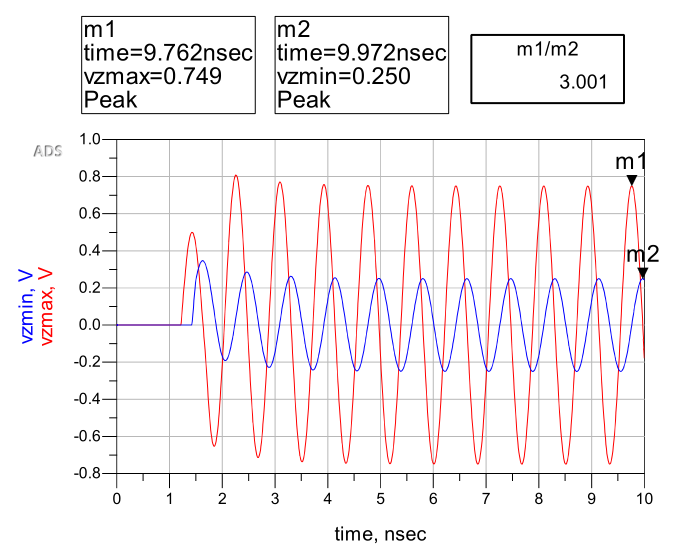
\includegraphics[width=9cm]{images/lab1_p3_vswr.png}
\caption{Voltage at source and load with sinusoidal excitation.}
\label{ads:plot:vswr} 
\end{figure}

\subsection{Mathematical expression of voltage along the line}

Considering a lossless line ($\alpha = 0$), the voltage along the line takes the form:

\begin{center}
    $V(-z) = V^+ e^{-\gamma z} +V^- e^{+ \gamma z}$ \\ \vspace{1pt}
    $V(-z) = V^+ e^{-j\beta z} +V^- e^{+ j\beta z}$ \\ \vspace{1pt}
\end{center}
\begin{equation} \label{p3:expvolt1} 
     V(-z) = V^+ e^{+ j\beta z} (1 + \rho_L e^{-2j \beta z})
\end{equation}

At the source ($z=l$) the previous expression becomes as follow (also the voltage provided by the source is the one after the voltage drop at the source impedance):

\begin{equation} \label{p3:expvolt2}
    V(-l) = V^+ e^{+ j\beta l} (1 + \rho_L e^{-2j \beta l})  = V_S - Z_S I_S
\end{equation}

While the source current is the composition of the incident and reflected current:

\begin{center} 
    $I_S = I^+(-l) + I^-(-l) = \frac{V^+(-l) + V^-(-l)}{Z_0}$
\end{center}

The expression \ref{p3:expvolt2} becomes:

\begin{center} 
    $V(-l) = \frac{V^+ e^{+j\beta l}}{Z_0} (1- \rho_L e^{+2j \beta l})$
\end{center}

Then:

\begin{equation} \label{p3:expvolt5}
    V^+ = V_S e^{-j \beta l} [(1+\rho_L e^{-2j\beta l})+\frac{Z_S}{Z_0}(1-\rho_L e^{-2j\beta l})]^{-1}
\end{equation}

Once $V^+$ is a known value, the expression \ref{p3:expvolt1} will allow us to trace the voltage envelope with a variable $z$ that will limit the voltage at any point and any time of the line.

The mathematical expression for the voltage along the line was derived in the Display Window environment of ADS, resulting in the figure \ref{calculus}. Once the variables were stored in the ADS work space, the waveform from figure \ref{p3:waveform} could be plotted, resulting in the combination of the upper and lower voltage envelope due to the stationary wave and the voltage waveform across the line in a given time (selected in a slider) bounded inside the envelope. Even varying the time instant of analysis, the voltage still bounded inside the envelope across all line.

\begin{figure}[H] 
\centering
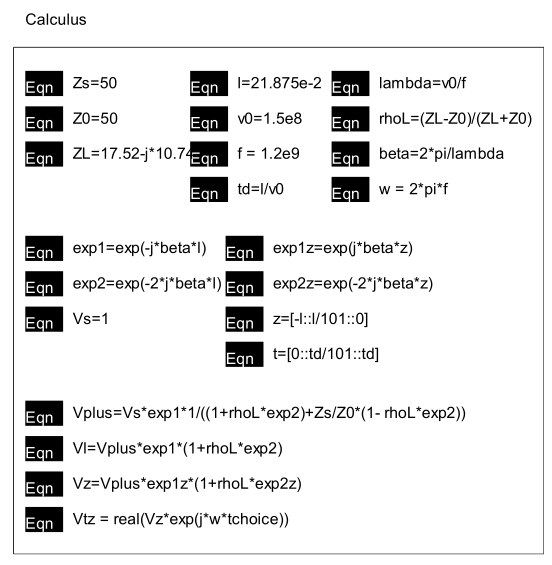
\includegraphics[width=9cm]{images/calculus.png}
\caption{Set of equations in the Display Window environment of ADS.}
\label{calculus} 
\end{figure}

\begin{figure}[H] 
\centering
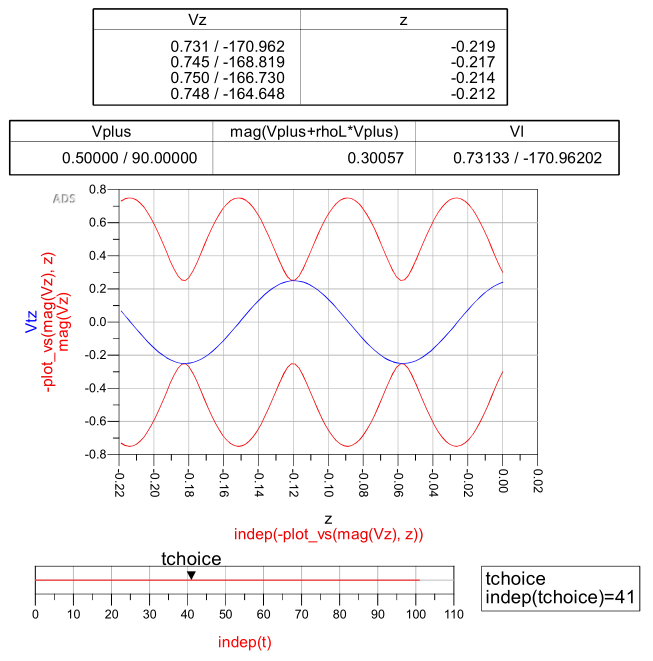
\includegraphics[width=12cm]{images/lab1_p3_waveform.png}
\caption{Waveform for the voltage along the line.}
\label{p3:waveform} 
\end{figure}
\section{Problem 4}

This problem consists in the analysis of the scattering parameters for a common-emitter amplifier with BC549 as seen in figure \ref{p3:bc549}.

\begin{figure}[H] 
\centering
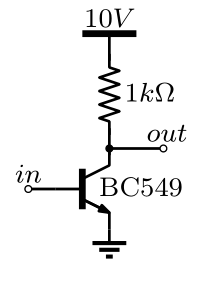
\includegraphics[width=3.5cm]{images/bc549.png}
\caption{Common-emitter amplifier with a bipolar junction transistor BC549.}
\label{p3:bc549} 
\end{figure}

The circuit above was simulated via ADS with the conditions below:

\begin{itemize}
    \item BJT polarized with $675 mV$;
    \item Source and load impedance of $Z_L = Z_S = 50 \Omega$;
    \item S-parameters simulation with frequency sweep between $1 kHz$ and $1 GHz$;
\end{itemize}

The ADS allow us to plot the behavior of each one of the scattering parameters considering 2 ports as seen in figure \ref{p4:sparams}.

\begin{figure}[H] 
\centering
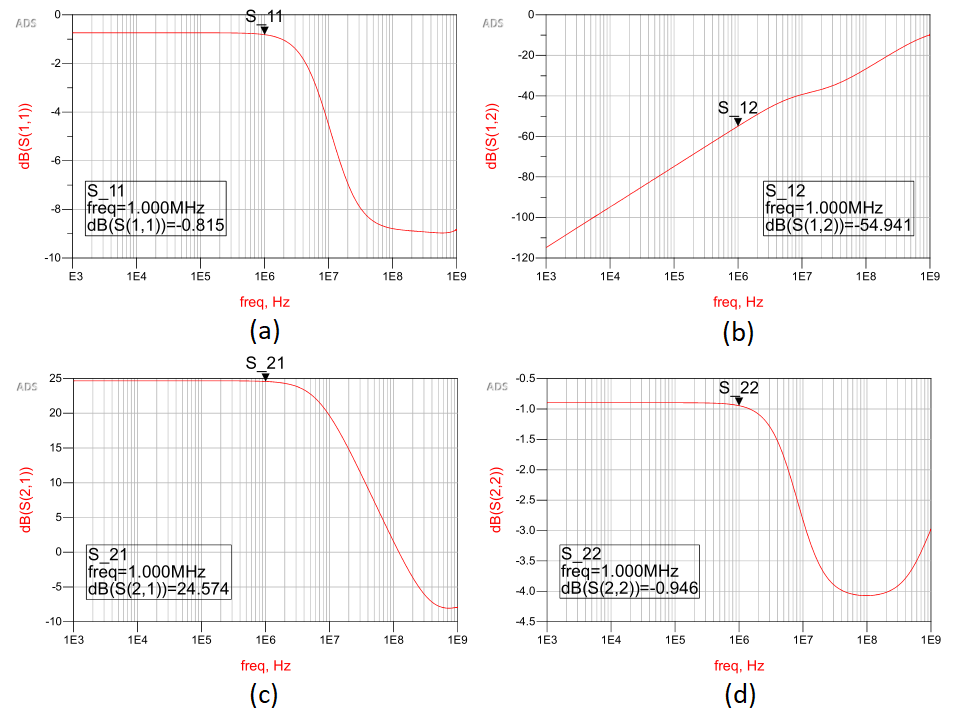
\includegraphics[width=15cm]{images/sparams.png}
\caption{Common-emitter amplifier with BC549 scattering parameters magnitude: (a) $s_{11}$, (b) $s_{12}$, (c) $s_{21}$ and (d) $s_{22}$.}
\label{p4:sparams} 
\end{figure}

Regarding the parameters $s_{11}$ and $s_{22}$ that denote the reflection coefficient in each port, we can observe by its magnitudes that they exert an approximately constant influence (but different between them) until the frequency of $1 MHz$. For higher frequencies the values tend to reduce, meaning that the reflected waves with these frequencies will be less influential. Regarding the other parameters their behavior are quiet different. The magnitude of $s_{21}$ (portion of the available power at the source [port 1] that was actually delivered to the load [port 2]) keeps approximately constant until $1 MHz$ and then drops. The behavior of $s_{11}$ and $s_{22}$ beyond $1 MHz$ are acceptable, but the effort is meaningless because of $s_{21}$, meaning that the reflected power is reduced as the transmitted power too. 

Once the circuit is not symmetrical, all the parameters will differ. The parameter $s_{12}$ have the oddest behavior, because it keeps risen but with no significant magnitude, meaning that the power flow from collector to base is nearly null but will rise due to the leakage current from the semiconductor junction reversed biased.

\subsection{Transducer power gain vs. Power gain}

The standard power gain is the relation between the output power (load power) with the input power $G_P = P_L/P_{in}$. But this relation does not take into account the power related to the reflected wave in the input port. So another metric is the transducer power gain the relates the output power with the total power available at the source $G_T = P_L/P_{av,s}$. So this allow us to analyse the maximum power gain at a impedance match situation.

Considering that the load power is $P_L = P_{av,s} \times |s_{21}|^2$ it is clear to see that the transducer power gain is simply the equation \ref{p4:gt}. Once the input power will be the available power at the source deducted the reflection losses: $P_{in} = P_{av,s} - P_r$. The power reflected at port 1 is $P_r = P_{av,s} \times |s_{11}|^2$. Replacing the reflected power and the available power as a function of $P_{av,s} = P_L / |s_{21}|^2$ we obtain a expression that depends only on the scattering parameters for the power gain in the equation \ref{p4:gp}. The expression also shows that in a condition without reflection ($s_{11} = 0$) both the gains are equals.

\begin{equation} \label{p4:gt}
    G_T = \frac{P_L}{P_{av,s}} = |s_{21}|^2
\end{equation}

\begin{equation} \label{p4:gp}
    G_P = \frac{P_L}{P_{in}} = \frac{|s_{21}|^2}{1 - |s_{11}|^2}
\end{equation}

In the previous simulation with load and source impedance of $50 \Omega$ and frequency of $100 MHz$, we can see by the plot of figure \ref{p4:gpgt} that $G_P = 1.648$ and $G_T = 1.43$. Since $s_{11}$ is lower than the unit for each and all frequencies of the plot, it results in $G_P > G_T$ and this is a coherent result because $P_{av,s} > P_{in}$, remembering that the available power incorporates the input power and the losses.


\begin{figure}[H] 
\centering
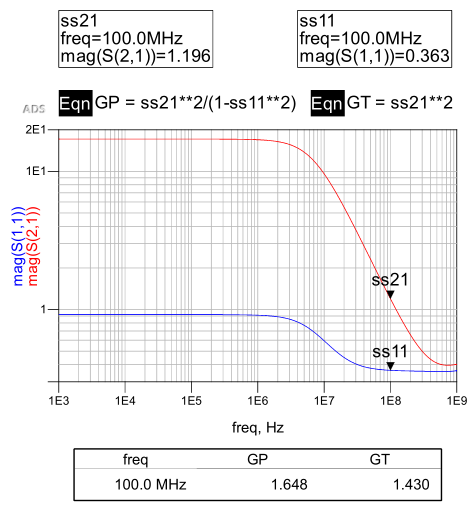
\includegraphics[width=9cm]{images/gpgt.png}
\caption{Common-emitter amplifier with BC549 transducer power gain ($G_T$) and power gain ($G_P$) at $100 MHz$.}
\label{p4:gpgt} 
\end{figure}

A practical way to prove this result is to feed the amplifier with a sine voltage of $1 mV_p$ and $100 MHz$ (same conditions of load and source impedance, polarization and transistor model) and check the power values. According to figure \ref{p4:gtproof} the resulting gain is $G_T = 1.395$. It differs from the previous result because the latter was found by a transient simulation with a limited time step that reduces precision and has convergence problems and the other was found via a simulation of S-parameters in a single point of frequency.

\begin{figure}[H] 
\centering
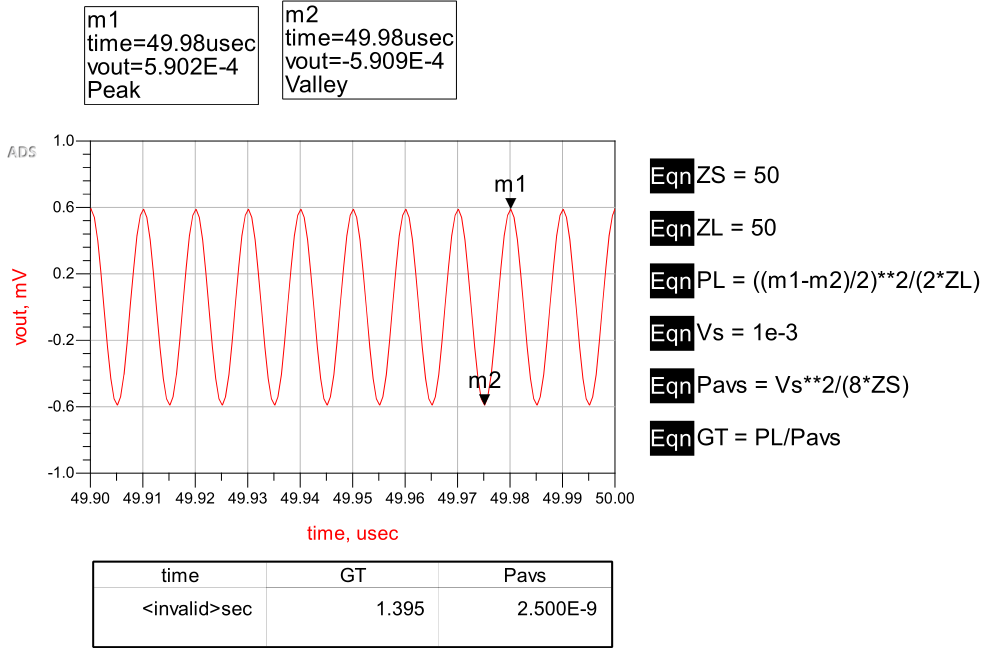
\includegraphics[width=13cm]{images/gtproof.png}
\caption{Proof of common-emitter amplifier with BC549 transducer power gain ($G_T$) at $100 MHz$.}
\label{p4:gtproof} 
\end{figure}

Another way to observe the transducer power gain is via a harmonic balance simulation at $100 MHz$. In this case it will not be used the circuit with the BJT, but a two ports generic quadripole characterized by the S-parameters founded before. The figure \ref{p4:Sparamcheck} show the SParamChecker for the generic quadripole of which the S-parameters sampled at $100 MHz$ matches the parameters obtained in the previous circuit like in figure \ref{p4:sparams}.

\begin{figure}[H] 
\centering
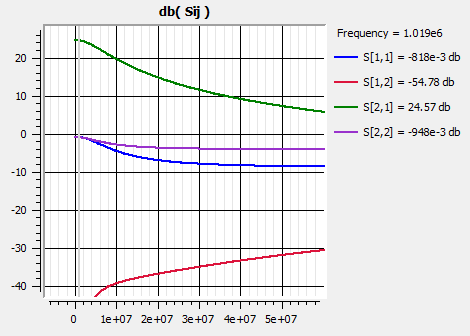
\includegraphics[width=9cm]{images/SParamChecker.png}
\caption{SParamChecker for generic quadripole.}
\label{p4:Sparamcheck} 
\end{figure}

Extracting the time domain signal from the load voltage in the harmonic balance (HB) simulation we observe the graphic in the figure \ref{p4:HB}. Despite feeding the quadripole with a $100 MHz$ sinusoidal voltage like in the previous simulation, the result for the transducer power gain differs from the previous simulations. 

\begin{figure}[H] 
\centering
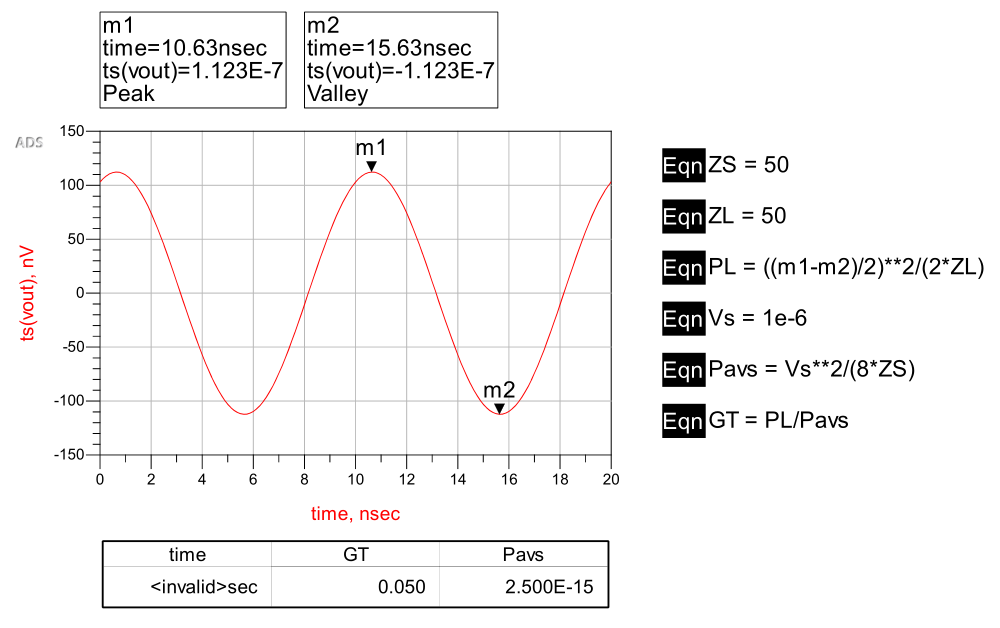
\includegraphics[width=12cm]{images/HB.png}
\caption{Time domain signal from HB simulation.}
\label{p4:HB} 
\end{figure}

This problem might have occurred due to maladjustments in the circuit parameters.


\end{document} 

